\documentclass{article}
\usepackage[utf8]{inputenc}
\usepackage{amsmath}
\usepackage{graphicx}
\usepackage{titling}

\title{\textbf{\Huge NLP Assignment 1: Answers}}
\author{Name: Alireza Dastmalchi Saei}
\date{Stu No.: 993613026}

\pretitle{%
  \begin{center}
  
\includegraphics[width = 150px]{Images/university-of-isfahan-logo.png}\\[\bigskipamount]
  \vspace{3cm}
}
\posttitle{\end{center}}

\begin{document}
\maketitle

\pagebreak

\section*{Question 1}
The 4 stages of natural languages are:
\begin{itemize}
    \item \textbf{Acoustic Ambiguity}: This type of ambiguity arises when words or phrases sound similar but have different meanings when put together. It occurs due to homophones or words with similar phonetic properties. Example:

        \begin{figure}[h]
          \centering
          
\includegraphics[width=1\textwidth]{Images/Acoustic.png}
          \label{fig:model_diagram}
        \end{figure}

    \item \textbf{Syntactic Ambiguity}: Syntactic ambiguity occurs when the structure or arrangement of words in a sentence allows for multiple interpretations. This ambiguity arises from the grammar or syntax of the language. Different parsing or grouping of words within the sentence can lead to distinct meanings. Example:
        \begin{figure}[h]
          \centering
          
\includegraphics[width=1\textwidth]{Images/Syntactic.png}
          \label{fig:model_diagram}
        \end{figure}

    \item \textbf{Semantic Ambiguity}: Semantic ambiguity involves words or phrases that have multiple meanings or interpretations based on context. This ambiguity arises from the ambiguity of individual words or phrases themselves, rather than the structure of the sentence. The meaning of the word may change depending on the context in which it is used. Example:
        \begin{figure}[h]
          \centering
          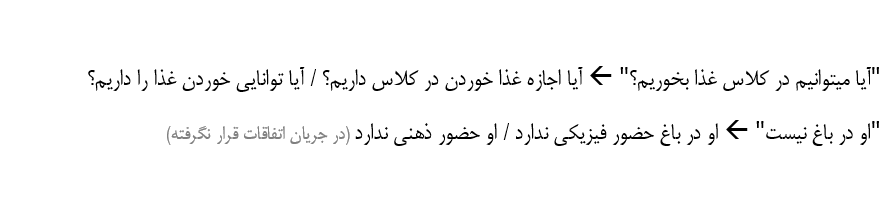
\includegraphics[width=1\textwidth]{Images/Semantic.png}
          \label{fig:model_diagram}
        \end{figure}

    \item \textbf{Discourse Ambiguity}: Discourse ambiguity refers to ambiguity that arises at the level of larger units of language, such as conversations, paragraphs, or entire texts. This type of ambiguity often arises when pronouns or other referring expressions lack clear antecedents or when there are ambiguities in the overall context of the communication. Example:
        \begin{figure}[h]
          \centering
          
\includegraphics[width=1\textwidth]{Images/Discourse.png}
          \label{fig:model_diagram}
        \end{figure}

\end{itemize}
\pagebreak

\section*{Question 2}
\textbf{Explanation}: The Maximum Matching Algorithm is a method used in Natural Language Processing (NLP) and text processing to segment words or tokens from a sequence of characters. It tries to find the longest possible sequences of words or tokens from the input text based on a given dictionary or vocabulary.\\\\
This algorithm takes a sequence of characters (string) as input. Then, using a list of all valid words available (dictionary), the algorithm iterates over the input text and tries to match the longest possible sequence of characters with words or tokens from the dictionary. This greedy algorithm returns a list of words or tokens segmented from the input text.\\\\
\textbf{Example}: This algorithm acts as follows:

\begin{figure}[h]
  \centering
  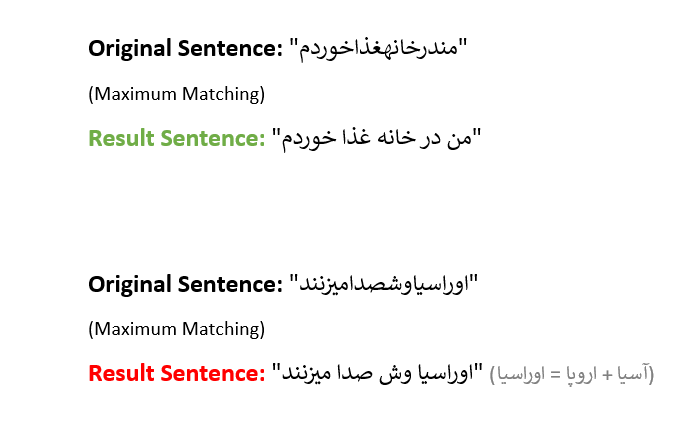
\includegraphics[width=1\textwidth]{Images/MaxMatch.png}
  \caption{Maximum Matching Example}
  \label{fig:model_diagram}
\end{figure}

\textbf{Applications}: Applications of the Maximum Matching Algorithm:
\begin{itemize}
  \item Tokenization in Natural Language Processing.
  \item Segmenting words or tokens from raw text in Information Retrieval systems.
  \item Word segmentation in languages without clear word boundaries, such as Chinese or Thai.
\end{itemize}

\pagebreak

\section*{Question 3}
\textbf{Lemmatization:} Lemmatization is the process of reducing words to their base or dictionary form, known as the lemma. It involves identifying the root form of a word considering its meaning. \\\\
\textbf{Stemming:} Stemming is the process of removing suffixes or prefixes from words to extract their root form, known as the stem. It's a heuristic process that chops off ends of words based on common patterns. However this method is not always able to produce valid dictionary words.

\begin{figure}[h]
  \centering
  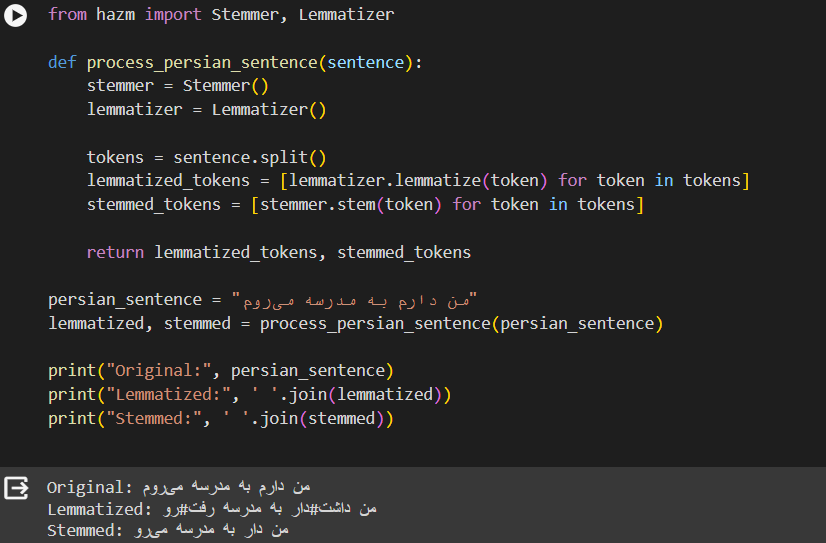
\includegraphics[width=1\textwidth]{Images/Stem_Lemma.png}
  \caption{Stemmed and Lemmatized}
  \label{fig:model_diagram}
\end{figure}

\end{document}
